\documentclass{beamer}

\mode<presentation> {
  \usetheme{Warsaw}
  \usefonttheme[onlylarge]{structuresmallcapsserif}
  \usefonttheme[onlysmall]{structurebold}
  \usecolortheme[overlystylish]{albatross}
  \setbeamercovered{transparent}
}


\usepackage[english]{babel}
\usepackage[latin1]{inputenc}
\usepackage{alltt}
\usepackage{amsmath}
\usepackage{amssymb}
\usepackage{amsmath,amssymb,amsfonts}
\usepackage{times}
\usepackage{multimedia}
\usepackage[T1]{fontenc}
\usepackage{graphicx}
\usepackage{subfigure}
\newcommand{\xieti}{\textsl}
\newcommand{\cuti}{\bfseries}
\newcommand{\huati}{\mathcal}

\title[]
{The Belief Propagation Decoding of LDPC Codes}


\author[]
{
Chaonian Guo\\
 \quad\\
\scriptsize{CIS Lab, Coding Group } }

\date
{Jan 9, 2009}

\subject{Talks}

\AtBeginSection[] {
  \begin{frame}<beamer>
    \frametitle{Outline}
    \tableofcontents[currentsection]
  \end{frame}
}

\AtBeginSubsection[] {
  \begin{frame}<beamer>
    \frametitle{Outline}
    \tableofcontents[currentsection,currentsubsection]
  \end{frame}
}


\begin{document}

\begin{frame}
  \titlepage
\end{frame}

\begin{frame}
  \frametitle{outline}
  \tableofcontents
\end{frame}

% =======================================   Begin  ======================================= %
% =======================================  section1 =========================================%
\section{About LDPC Codes}

\subsection{Research aspects}

\begin{frame}{Research aspects}
    \begin{itemize}
    \item Coding: \xieti{H}.
    \item Decoding: simplification\&accuracy of decoding.
    \item Density Evolution: improvements.
    \item Design of Irregular LDPC Codes: degree distribution.
    \item Distance\&Performance: analysis.
    \item Implementation\&Application: communication.
    \end{itemize}
\end{frame}

\subsection{Basic Conceptions}
\begin{frame}
    \begin{block}{LDPC Codes}
        A binary Low-Density Parity-Check code, specified by a parity check matrix
        \xieti{H$_{(N-K)\times N}$} in \xieti{GF(2)}: the 0's are far more than the 1's.
        \begin{itemize}
            \item \xieti{N}: the linear block length of a codeword \xieti{c}.
            \item \xieti{K}: the length of the source \xieti{s}.
            \item \xieti{M}: the number of check bits ($M = N-K$).
            \item \xieti{R}: code rate = $\frac{K}{N}$.
            \item \xieti{G$_{K\times N}$}: generator matrix specified by \xieti{G$^T$H} = \xieti{0}.
        \end{itemize}
    \end{block}
\end{frame}

\begin{frame}
    \begin{block}{Example 1}
        The parity check matrix of a trivial LDPC code may be
        \[
            \xieti{H}=
            \left[
            \begin{array}[]{cccccc}
            1 & 1 & 0 & 1 & 0 & 0 \\
            0 & 1 & 1 & 0 & 0 & 1 \\
            1 & 0 & 1 & 0 & 1 & 0
            \end{array}
            \right],
        \]\\
        which means:
        \begin{equation*}
            \left\{
            \begin{aligned}
            \xieti{c$_1$+c$_2$+c$_4$} = 0\\
            \xieti{c$_2$+c$_3$+c$_6$} = 0\\
            \xieti{c$_1$+c$_3$+c$_5$} = 0
            \end{aligned} \right.
        \end{equation*}
    \end{block}
\end{frame}

\begin{frame}
    \begin{block}{Regular \& Irregular LDPC Codes}
        \begin{itemize}
            \item(\xieti{d$_v$},  \xieti{d$_c$})-regular codes
                \begin{itemize}
                    \item All the column weights are \xieti{d$_v$}.
                    \item All the row weights are \xieti{d$_c$}.
                \end{itemize}
            \item ($\lambda(x), \rho(x)$)-irregular codes
                \begin{itemize}
                    \item  $\lambda(x) = \sum \lambda_ix^{i-1}$, $\rho(x) = \sum \rho_ix^{i-1}$.
                    \item $\lambda_i$: the fraction of columns of weight \xieti{i} in \xieti{H}.
                    \item $\rho_i$: the fraction of rows of weight \xieti{i} in \xieti{H}.
                \end{itemize}
        \end{itemize}
    \end{block}
\end{frame}

\begin{frame}
    \begin{block}{Example 2}
    \begin{itemize}
        \item (2,4)-regular LDPC code:
        \[
            \xieti{H}=
            \left[
            \begin{array}[]{cccccccccc}
            1 & 1 & 1 & 1 & 0 & 0 & 0 & 0 & 0 & 0\\
            1 & 0 & 0 & 0 & 1 & 1 & 1 & 0 & 0 & 0\\
            0 & 1 & 0 & 0 & 1 & 0 & 0 & 1 & 1 & 0\\
            0 & 0 & 1 & 0 & 0 & 1 & 0 & 1 & 0 & 1\\
            0 & 0 & 0 & 1 & 0 & 0 & 1 & 0 & 1 & 1\\
            \end{array}
            \right].
        \]\\
        \item ($\lambda(x), \rho(x)$)-irregular LDPC code, $\lambda(x)=0.4x+0.6x^2$, $\rho(x)=0.2x^2+0.8x^3:$
        \[
            \xieti{H}=
            \left[
            \begin{array}[]{cccccc}
            1 & 1 & 1 & 0 & 1 & 0 \\
            1 & 0 & 1 & 1 & 0 & 1 \\
            0 & 0 & 1 & 1 & 1 & 1 \\
            0 & 1 & 0 & 1 & 0 & 1
            \end{array}
            \right].
        \]\\
    \end{itemize}
    \end{block}
\end{frame}


\subsection{Coding \& Decoding Process}
\begin{frame}
    \begin{block}{Coding \& Decoding Process}
        \begin{itemize}
        \item Source sequence \xieti{s} = \{\xieti{s$_1$, s$_2$, ..., s$_K$}\}.
        \item Code by \xieti{s$\cdot$G} $\rightarrow$ codeword \xieti{c} = \{\xieti{c$_1$, c$_2$, ..., c$_N$}\}.
        \item Modulate codeword \xieti{c} $\rightarrow$ \xieti{x}.
        \item Transmit \xieti{x}.
        \item Receive \xieti{x} and demodulate \xieti{x} $\rightarrow$ \xieti{y}.
        \item Decode \xieti{y} $\rightarrow$ codeword \xieti{$\hat{c}$}.
        \end{itemize}
    \end{block}
\end{frame}
\begin{frame}
    \begin{block}{Decoding}
        Giving \xieti{y}, how to determine \xieti{$\hat{c}$}?
        \begin{itemize}
            \item Hard decision decoding: Bit-Flip.
            \item Soft decision decoding: Belief Propagation.
        \end{itemize}
    \end{block}
\end{frame}

% =======================================  section2 =========================================%
\section{The BP Decoding of LDPC Codes}

\subsection{Posteriori Probability}
\begin{frame}
    \begin{block}{Posteriori Probability}
        The \xieti{Posteriori Probability} of the codeword \xieti{c} is
        computed based on the received value \xieti{y} .\\
        \quad \\
        \quad The \xieti{d$^{\;th}$} bit c$_d$:
        \begin{itemize}
        \item Pr(\xieti{c$_d$ = 0}$|y_d$, \xieti{S}), Pr(\xieti{c$_d$ = 1}$|y_d$, \xieti{S}).
        \item \xieti{S}: bit \xieti{c$_d$} satisfies all the check equations.
        \end{itemize}
    \end{block}
\end{frame}
\begin{frame}
    \begin{block}{Lemma}
        Consider a sequence of \xieti{m} independent binary digits in
        which the \xieti{l$^{\;th}$} digit is a 1 with probability
        \xieti{P$_l$}. Then the probability that an even number of
        digits are 1 is $\frac{1 + \prod_{l=1}^{m}{(1-2P_l)}}{2}$.
    \end{block}
\end{frame}
\begin{frame}
    \begin{block}{Theorem}
        Let \xieti{P$_d$} be the probability that \xieti{c$_d$} is a 1 conditional on
        the received digit \xieti{y$_d$}, and let \xieti{P$_{il}$} be same probability
        for the \\\xieti{l$^{\; th}$} bit in the \xieti{i$^{\; th}$} check equation. Let
        the digits be statistically independent of each other. Then\\
        \begin{center}
        $\frac{Pr(c_d = 0|y_d, S)}{Pr(c_d = 1|y_d, S)}$ = $\frac{1-P_d}{P_d}$
        $\prod_{i=1}^{d_v}$
        $\frac{1+\prod_{l=1}^{d_c-1}(1-2P_{il})}{1-\prod_{l=1}^{d_c-1}(1-2P_{il})}$
        \end{center}
    \end{block}
\end{frame}
\begin{frame}
    \begin{block}{Proof}
        \Large{
          $\frac{Pr(c_d = 0|y_d, S)}{Pr(c_d = 1|y_d, S)}$\\
        = $\frac{Pr(c_d=0,y_d,S)/Pr(y_d,S)}{Pr(c_d=1,y_d,S)/Pr(y_d,S)}$\\
        = $\frac{Pr(c_d=0,y_d,S)}{Pr(c_d=1,y_d,S)}$\\
        = $\frac{Pr(y_d)Pr(c_d=0|y_d)Pr(S|c_d=0,y_d)}{Pr(y_d)Pr(c_d=1|y_d)Pr(S|c_d=1,y_d)}$\\
        = $\frac{1-P_d}{P_d}\prod_{i=1}^{d_v}\frac{(1+\prod_{l=1}^{d_c-1}(1-2P_{il}))/2}{(1-\prod_{l=1}^{d_c-1}(1-2P_{il}))/2}$\\
        = $\frac{1-P_d}{P_d}\prod_{i=1}^{d_v}\frac{1+\prod_{l=1}^{d_c-1}(1-2P_{il})}{1-\prod_{l=1}^{d_c-1}(1-2P_{il})}$
        }\quad \quad \quad \quad \quad \quad \quad \quad \quad $\square$
    \end{block}
\end{frame}

\subsection{Belief Propagation}
\begin{frame}
    \begin{block}{Notations}
        \begin{itemize}
        \item N(m): \{n|\xieti{H$_{mn}$=1,1$\leq n\leq N$}\}.
        \item M(n): \{m|\xieti{H$_{mn}$=1,1$\leq m\leq M$}\}.
        \item r$_{mn}$(0): the probability of check \xieti{m} being satisfied when bit \xieti{n} is 0.
        \item r$_{mn}$(1):\quad...
        \item q$_{mn}$(0): the probability that bit \xieti{n} has the value 0, given the information obtained by the checks other than check \xieti{m}.
        \item q$_{mn}$(1):\quad...
        \item q$_{n}$(0): the probability that bit \xieti{n} has the value 0, given the information obtained by all the checks.
        \item q$_{n}$(1): \quad...
        \end{itemize}
    \end{block}
\end{frame}
\begin{frame}
    \begin{block}{Decoding Process(1)}
        \begin{itemize}
        \item Initialization: \begin{equation*}q_{mn}^{(0)}(0)=P_i(0), q_{mn}^{(0)}(1)=P_i(1), t=1\end{equation*}
        \item Updating check node messages: \begin{equation*}
                                            r_{mn}^{(t)}(0)=\frac{1}{2}+\frac{1}{2}\prod_{n^\prime\in N(m)\backslash n}
                                            (1-2q_{mn^\prime}^{(t-1)}(1))
                                            \end{equation*}
                                            \begin{equation*}
                                            r_{mn}^{(t)}(1)=\frac{1}{2}-\frac{1}{2}\prod_{n^\prime\in N(m)\backslash n}
                                            (1-2q_{mn^\prime}^{(t-1)}(1))
                                            \end{equation*}
        \end{itemize}
    \end{block}
\end{frame}
\begin{frame}
    \begin{block}{Decoding Process(2)}
        \begin{itemize}
        \item Updating variable node messages:\begin{equation*}
                                              q_{mn}^{(t)}(0)=P_n(0)\prod_{m^\prime\in M(n)\backslash m}r_{m^\prime n}^{(t)}(0)
                                              \end{equation*}
                                              \begin{equation*}
                                              q_{mn}^{(t)}(1)=P_n(1)\prod_{m^\prime\in M(n)\backslash m}r_{m^\prime n}^{(t)}(1)
                                              \end{equation*}
        \end{itemize}
    \end{block}
\end{frame}
\begin{frame}
    \begin{block}{Decoding Process(3)}
        \begin{itemize}
        \item Decoding:\begin{equation*}
                                              q_{n}^{(t)}(0)=P_n(0)\prod_{m\in M(n)}r_{mn}^{(t)}(0)
                                              \end{equation*}
                                              \begin{equation*}
                                              q_{n}^{(t)}(1)=P_n(1)\prod_{m\in M(n)}r_{mn}^{(t)}(1)
                                              \end{equation*}
                                              \begin{itemize}
                                              \item if q$_{n}^{(t)}$(0) $>$ q$_{n}^{(t)}$(1), then $\hat{c}_n$ = 0;
                                              \item else $\hat{c}_n$ = 1.
                                              \end{itemize}
        \end{itemize}
    \end{block}
\end{frame}
\begin{frame}
    \begin{block}{Decoding Process(4)}
        \begin{itemize}
        \item Stopping criterion test:
            \begin{itemize}
            \item if \xieti{H}$\hat{c}$ = \xieti{0}, then the decoding process ends;
            \item if \xieti{t} exceeds some maximum number, and $\hat{c}$ is considered as the final codeword, then the process ends;
            \item otherwise, continue the iteration.
            \end{itemize}
        \end{itemize}
    \end{block}
\end{frame}

\subsection{LLR BP}

\begin{frame}{Log-likelihood Belief Propagation}
    \begin{block}{identical equation}
        tanh($\frac{1}{2}$ln$\frac{p_0}{p_1}$) = $p_0-p_1=1-2p_1$.
        \\($p_0+p_1$ = 1,tanh(x) = $\frac{e^x-e^{-x}}{e^x+e^{-x}}$)
    \end{block}
    \begin{block}{LLR}
            $r_{mn}^{(t)}(1)=\frac{1}{2}-\frac{1}{2}\prod_{n^\prime\in N(m)\backslash n}(1-2q_{mn^\prime}^{(t-1)}(1))$\\
            $\Rightarrow$ 1-2$r_{mn}^{(t)}(1)=\prod_{n^\prime\in N(m)\backslash n}(1-2q_{mn^\prime}^{(t-1)}(1))$\\
            $\Rightarrow $ tanh($\frac{1}{2}$ln$\frac{r_{mn}^{(t)}(0)}{r_{mn}^{(t)}(1)}$)=$\prod_{n^\prime\in N(m)\backslash n}$tanh($\frac{1}{2}$ln$\frac{q_{mn^\prime}^{(t-1)}(0)}{q_{mn^\prime}^{(t-1)}(1)}$)
    \end{block}
\end{frame}
\begin{frame}
    \begin{block}{LLR BP}
        \begin{equation}
        ln\frac{r_{mn}^{(t)}(0)}{r_{mn}^{(t)}(1)}=2tanh^{-1}(\prod_{n^\prime\in N(m)\backslash
        n}tanh(\frac{1}{2}ln\frac{q_{mn^\prime}^{(t-1)}(0)}{q_{mn^\prime}^{(t-1)}(1)}));
        \end{equation}
        \begin{equation}
        ln\frac{q_{mn}^{(t)}(0)}{q_{mn}^{(t)}(1)}=ln\frac{P_n(0)}{P_n(1)}+\sum_{m^\prime\in M(n)\backslash
        m}ln\frac{r_{m^\prime n}^{(t)}(0)}{r_{m^\prime n}^{(t)}(1)}.
        \end{equation}
    \end{block}
\end{frame}
% =======================================  section3 =========================================%
\section{Some Improved Results}

\subsection{Fluctuations}
\begin{frame}
    \begin{block}{The variable node LLR}
        The variable node LLR fluctuates continously during the iterative
        decoding:
        \begin{itemize}
        \item \quad...
        \item ln$\frac{q_{mn}^{(t-1)}(0)}{q_{mn}^{(t-1)}(1)}>0 \;(<0);$
        \item ln$\frac{q_{mn}^{(t)}(0)}{q_{mn}^{(t)}(1)}<0 \;(>0);$
        \item ln$\frac{q_{mn}^{(t+1)}(0)}{q_{mn}^{(t+1)}(1)}>0 \;(<0);$
        \item \quad...
        \end{itemize}
    \end{block}
\end{frame}

\subsection{Adaptive Erasure}
\begin{frame}
    \begin{block}{CFT}
        Introduce a sequence of counters to record the Continuous
        Fluctuant Times (CFT) of the variable node LLRs:
        \begin{equation*}
        {CFT_{mn}^{(t)}=}
            \begin{cases}
            0; & t=0;\\
            CFT_{mn}^{(t-1)}+1 ;& ln\frac{q_{mn}^{(t-1)}(0)}{q_{mn}^{(t-1)}(1)}\cdot ln\frac{q_{mn}^{(t)}(0)}{q_{mn}^{(t)}(1)}<0;\\
            0 ;& otherwise.\\
            \end{cases}
        \end{equation*}
    \end{block}
\end{frame}
\begin{frame}
    \begin{block}{Erase the LLRs}
        \large{
        \begin{equation*}
        {ln\frac{q_{mn}^{(t)}(0)}{q_{mn}^{(t)}(1)}=}
            \begin{cases}
            \quad\quad\quad 0 ;& CFT_{mn}^{(t)} \geq 2;\\
            ln\frac{q_{mn}^{(t-1)}(0)}{q_{mn}^{(t-1)}(1)}+ln\frac{q_{mn}^{(t)}(0)}{q_{mn}^{(t)}(1)};& CFT_{mn}^{(t)}=1;\\
            \quad \quad\quad ln\frac{q_{mn}^{(t)}(0)}{q_{mn}^{(t)}(1)} ;& otherwise.
            \end{cases}
        \end{equation*}}
    \end{block}
\end{frame}

\subsection{Simulation Results}
\begin{frame}{Simulation Results}
    \begin{center}
    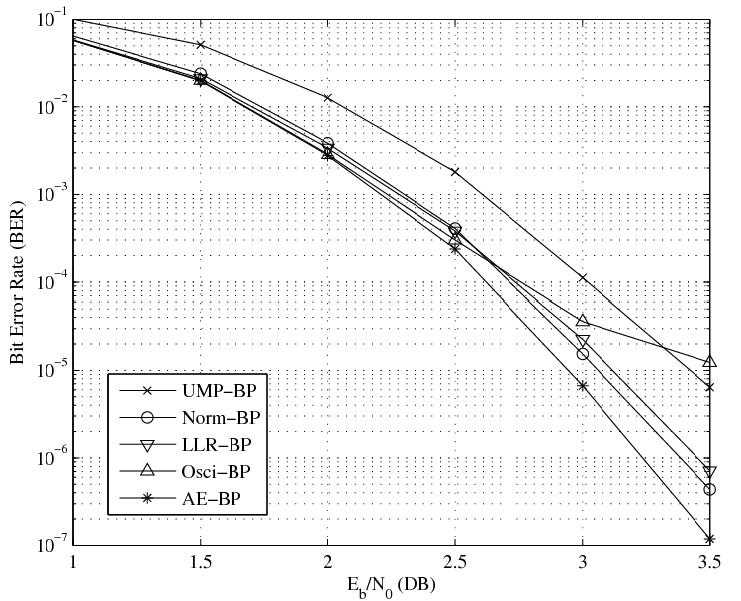
\includegraphics[width=2.5in]{ber252.jpg}\\
    Error performances for iterative decoding, \\(3,6)-regular LDPC code with N=504 and R=1/2.
    \end{center}
\end{frame}
% =======================================  section4 =========================================%
\section{The End: Literature Review}
\begin{frame}{Main Progress}
    \begin{itemize}
    \item Gallager, 1963: first proposed LDPC codes.
    \item Tanner, 1981: modeled the decoding process by  Tanner Graph.
    \item Mackay\&Neal, 1996: rediscovered LDPC codes.
    \item Luby, 1997: proposed irregular LDPC codes.
    \item Richardson\&Urbanke, 2001: Density Evolution and code threshold.
    \item S.-Y Chung, 2001: within 0.0045dB of the Shannon Limit by Gaussian Approximation.
    \item M. Ardakani, 2004: semi-Gaussian Approximation.
    \item Now: Over \xieti{GF(q)} \& Quasi-cyclic LDPC Codes.
    \end{itemize}
\end{frame}
\begin{frame}{LDPC Codes Decoding}
    \begin{block}{BP}
        \begin{itemize}
        \item BP, LLR-BP (SPA).
        \item UMP-BP: Fossorier 1999.
        \item Normalized/Offset BP: J. Chen 2002.
        \item BP based on Oscillation: S. Gounai 2006.
        \end{itemize}
    \end{block}
    \begin{block}{Bit-Flip}
        \begin{itemize}
        \item ...
        \end{itemize}
    \end{block}
    \begin{block}{Next}
        Storage $\leftrightarrow$ Error Correcting Code
    \end{block}
\end{frame}
\begin{frame}
    \begin{center}
        \huge{Thank you \\\& happy Niu year!}
    \end{center}
\end{frame}
% =======================================   END  =========================================%
\end{document}
